
\documentclass{article}
\usepackage{amsmath,amssymb,amsthm,latexsym,paralist}
\usepackage{graphicx}
\usepackage{verbatim}
\usepackage[a4paper, total={6in, 8in}]{geometry}
\usepackage{mathtools}
\DeclarePairedDelimiter{\ceil}{\lceil}{\rceil}
\usepackage{tikz}

\theoremstyle{definition}
\newtheorem{problem}{Problem}
\newtheorem*{solution}{Solution}
\newtheorem*{resources}{Resources}

\newcommand{\name}[1]{\noindent\textbf{Name: #1}}
\newcommand{\honor}{\noindent On my honor, as an Aggie, I have neither
  given nor received any unauthorized aid on any portion of the
  academic work included in this assignment. Furthermore, I have
  disclosed all resources (people, books, web sites, etc.) that have
  been used to prepare this homework. \\[1ex]
 \textbf{Signature:} \underline{\hspace*{5cm}} }

%  \newcommand{\checklist}{\noindent\textbf{Checklist:}
% \begin{compactitem}[$\Box$] 
% \item Did you add your name? 
% \item Did you disclose all resources that you have used? \\
% (This includes all people, books, websites, etc. that you have consulted)
% \item Did you sign that you followed the Aggie honor code? 
% \item Did you solve all problems? 
% \item Did you submit (a) the pdf file of your homework?
% \item Did you submit (b) a hardcopy of the pdf file in class? 
% \end{compactitem}
% }



\newcommand{\problemset}[1]{\begin{center}\textbf{Problem Set
      #1}\end{center}}
\newcommand{\duedate}[2]{\begin{quote}\textbf{Due dates:} Electronic
    submission of the pdf file of this homework is due on
    \textbf{#1} on ecampus, a signed paper copy of the pdf file is due
    on \textbf{#2} at the beginning of class. \end{quote} }

\newcommand{\N}{\mathbf{N}}
\newcommand{\R}{\mathbf{R}}
\newcommand{\Z}{\mathbf{Z}}


\begin{document}
\problemset{6}
\duedate{3/7/2019 before noon}{3/7/2019}
\name{ Hunter Cleary}
\begin{resources} (All people, books, articles, web pages, etc. that
  have been consulted when producing your answers to this homework)
  \begin{itemize}
      \item https://oeis.org/A004526/a004526.pdf
      \item https://stackoverflow.com/questions/9657756/graph-square-of-a-directed-graph
      \item https://www.cs.duke.edu/courses/fall05/cps130/lectures/skiena.lectures/lecture15.pdf
      \item https://www3.cs.stonybrook.edu/~algorith/video-lectures/1997/lecture15.pdf
      \item https://math.stackexchange.com/questions/1231144/what-is-the-special-of-product-of-the-incidence-matrix-and-its-transpose-for-an
      \item https://www.geeksforgeeks.org/breadth-first-search-or-bfs-for-a-graph/
  \end{itemize}
\end{resources}
\honor

\newpage

% Read chapter 22 in our textbook before attempting to answer these
% questions. 

\begin{problem}[20 points]
Solve Exercise 22.1-5 on page 593 of our textbook. 
\end{problem}
\begin{solution} \\
If the square of graph $G$ is $G^2$, then each entry $a^2_{ij}$ in adjacency matrix of G is 1, if vertices i and j are seperated by a single edge or two edges.
\begin{itemize}
\item An entry $a_{ij}$ in adjacenecy matrix A of G is 1, if there is an edge between two vertices i and j. Otherwise $a_{ij}$ is 0.
\item If A is multiplied itself and the result is matrix $A^2$, then each entry $a^2_{ij}$ in $A^2$ is 1, if there is a path of exactly 2 edges between i and j. Otherwise, $a^2_{ij}$ is 0
\item To obtain the adjacency matrix of a square of directed graph, merge the A and $A^2$ usch that each entry in the final adjacency matrix is 1, if vertices i and j are either separated by single edge or two edges.
\end{itemize}
\\
For Adjacency Matrix
\begin{itemize}
    \item The adjacenecy-list representation of a graph $G=(V,E)$ consists of an array of |V| lists, one for each vertex in V.
\end{itemize}
\begin{verbatim}
let G^2 be a new graph adjacenecy matrix A^2 = (a^2[i][j])
SquareDirectedGraph(){
    for(int i = 0 ; i < lengthof |V| ; i++){
        for (int j = 0 ; j < lengthof |V| ; j++){
            a[i][j] = 0;
            for((int k = 0 ; k < lengthof |V| ; k++){
                if ( a[i][k] = 1 && a[k][j] = 1 ){
                    A2[i][j] = 1;
                }
            }
        }
    }
}
\end{verbatim}
This algorithm runs in $O(n^3)$ where n is the length of $|V|$. It must loop the length of each row in the adjacency matrix.\\
\\
For Adjancency List
\begin{verbatim}
//using for in place of iterator
V[A2] = V[A];
for ( int i = 0 ; i < u in V[A] ; i++){
    for ( int i = 0 ; i < v in Adj[u] ; i++){
        for (int k = 0 ; k < w in Adj[u] ; k ++){
            E[G2] = {(u,w)} E[G2]
        }
    }
}
\end{verbatim}
This algorithm also runs in $O(n^3)$ where n is the length of $|V|$.\\

\end{solution}

\newpage

\begin{problem}[20 points]
Solve Exercise 22.1-7 on page 593 of our textbook. 
\end{problem}
\begin{solution} \\
\\
The incidence matrix of a directed graph $G = (v,E)$ with no self-loops is a $|V| x |E|$ matrix $B = B_{ij}$ such that:\\
\indent $b_{ij}= -1$ if edge j leaves vertex i\\
\indent $b_{ij}= \ \  1$ if edge j enters vertex i\\
\indent $b_{ij}= \ \ 0$ otherwise\\
Describe what the entries of the matrix product $BB^T$ represent, where $B^T$ is the transpose of B.\\
\\
$$a_{jk} = a^T_{kj}$$
$$b_{ij} = \sum_{k}^{} a_{ik}*a_{jk} $$ \\
$a_{ik}*a_{jk}$ is equal to 1 if vertices i and j are incident with edge k (0 otherwise). If i does not equal j, the entry counts the number of edges from vertex i to j.\\
\begin{equation}
    a_{ij}=
    \begin{cases}
      a_{ij}, & \text{if}\ i \ \ !=  \ \ j \\
      a_{ii}, & \text{if} i = j 
    \end{cases}
  \end{equation}
  So
  \begin{equation}
    a_{ij}=
    \begin{cases}
      a_{ij}, & \text{the number of edges incident to both }$V_i$ \text{and} $V_j$\\ 
      a_{ii}, & \text{the number of edges incident to} $V_{i}$
    \end{cases}
  \end{equation}

\end{solution}

\newpage

\begin{problem}[20 points]
Solve Exercise 22.2-6 on page 602. Use tikz to draw the graph in your
LaTeX document. 
\end{problem}
\begin{solution} \\
\\



\tikzset{every picture/.style={line width=0.75pt}} %set default line width to 0.75pt        

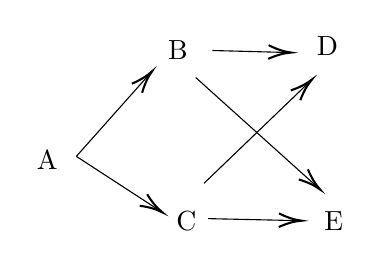
\begin{tikzpicture}[x=0.75pt,y=0.75pt,yscale=-1,xscale=1]
%uncomment if require: \path (0,193); %set diagram left start at 0, and has height of 193

%Straight Lines [id:da7671178109085042] 
\draw    (100,108) -- (135.17,68.49) ;
\draw [shift={(136.5,67)}, rotate = 491.68] [color={rgb, 255:red, 0; green, 0; blue, 0 }  ][line width=0.75]    (10.93,-3.29) .. controls (6.95,-1.4) and (3.31,-0.3) .. (0,0) .. controls (3.31,0.3) and (6.95,1.4) .. (10.93,3.29)   ;

%Straight Lines [id:da5752878963713413] 
\draw    (100,108) -- (139.82,133.91) ;
\draw [shift={(141.5,135)}, rotate = 213.05] [color={rgb, 255:red, 0; green, 0; blue, 0 }  ][line width=0.75]    (10.93,-3.29) .. controls (6.95,-1.4) and (3.31,-0.3) .. (0,0) .. controls (3.31,0.3) and (6.95,1.4) .. (10.93,3.29)   ;

%Straight Lines [id:da9848570747101226] 
\draw    (157.5,70) -- (216.01,122.66) ;
\draw [shift={(217.5,124)}, rotate = 221.99] [color={rgb, 255:red, 0; green, 0; blue, 0 }  ][line width=0.75]    (10.93,-3.29) .. controls (6.95,-1.4) and (3.31,-0.3) .. (0,0) .. controls (3.31,0.3) and (6.95,1.4) .. (10.93,3.29)   ;

%Straight Lines [id:da7032983241128152] 
\draw    (165.5,57) -- (201.5,57.95) ;
\draw [shift={(203.5,58)}, rotate = 181.51] [color={rgb, 255:red, 0; green, 0; blue, 0 }  ][line width=0.75]    (10.93,-3.29) .. controls (6.95,-1.4) and (3.31,-0.3) .. (0,0) .. controls (3.31,0.3) and (6.95,1.4) .. (10.93,3.29)   ;

%Straight Lines [id:da45735483996911785] 
\draw    (161.5,121) -- (212.06,72.39) ;
\draw [shift={(213.5,71)}, rotate = 496.12] [color={rgb, 255:red, 0; green, 0; blue, 0 }  ][line width=0.75]    (10.93,-3.29) .. controls (6.95,-1.4) and (3.31,-0.3) .. (0,0) .. controls (3.31,0.3) and (6.95,1.4) .. (10.93,3.29)   ;

%Straight Lines [id:da6040700762949336] 
\draw    (163.5,138) -- (206.5,138.96) ;
\draw [shift={(208.5,139)}, rotate = 181.27] [color={rgb, 255:red, 0; green, 0; blue, 0 }  ][line width=0.75]    (10.93,-3.29) .. controls (6.95,-1.4) and (3.31,-0.3) .. (0,0) .. controls (3.31,0.3) and (6.95,1.4) .. (10.93,3.29)   ;


% Text Node
\draw (86,110) node  [align=left] {A};
% Text Node
\draw (149,57) node  [align=left] {B};
% Text Node
\draw (153,139) node  [align=left] {C};
% Text Node
\draw (221,55) node  [align=left] {D};
% Text Node
\draw (224,139) node  [align=left] {E};


\end{tikzpicture}\\
\\
Performing BFS on the Graph\\
The graph with all edges cannot be replicated using breadth-first search. Using the starting node A, neighbor nodes B and C will be enqueued. The precedence of these nodes will not change the outcome. If B is precedent, it will be visited and nodes D and E will be enqueued. This will cause the edges CE and CD to be left out of the search. \\




\tikzset{every picture/.style={line width=0.75pt}} %set default line width to 0.75pt        

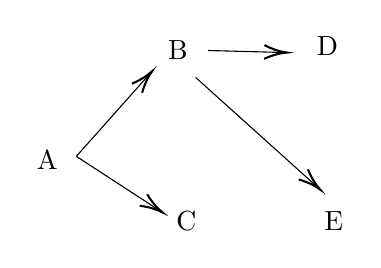
\begin{tikzpicture}[x=0.75pt,y=0.75pt,yscale=-1,xscale=1]
%uncomment if require: \path (0,193); %set diagram left start at 0, and has height of 193

%Straight Lines [id:da7671178109085042] 
\draw    (100,108) -- (135.17,68.49) ;
\draw [shift={(136.5,67)}, rotate = 491.68] [color={rgb, 255:red, 0; green, 0; blue, 0 }  ][line width=0.75]    (10.93,-3.29) .. controls (6.95,-1.4) and (3.31,-0.3) .. (0,0) .. controls (3.31,0.3) and (6.95,1.4) .. (10.93,3.29)   ;

%Straight Lines [id:da5752878963713413] 
\draw    (100,108) -- (139.82,133.91) ;
\draw [shift={(141.5,135)}, rotate = 213.05] [color={rgb, 255:red, 0; green, 0; blue, 0 }  ][line width=0.75]    (10.93,-3.29) .. controls (6.95,-1.4) and (3.31,-0.3) .. (0,0) .. controls (3.31,0.3) and (6.95,1.4) .. (10.93,3.29)   ;

%Straight Lines [id:da9848570747101226] 
\draw    (157.5,70) -- (216.01,122.66) ;
\draw [shift={(217.5,124)}, rotate = 221.99] [color={rgb, 255:red, 0; green, 0; blue, 0 }  ][line width=0.75]    (10.93,-3.29) .. controls (6.95,-1.4) and (3.31,-0.3) .. (0,0) .. controls (3.31,0.3) and (6.95,1.4) .. (10.93,3.29)   ;

%Straight Lines [id:da7032983241128152] 
\draw    (163.5,57) -- (199.5,57.95) ;
\draw [shift={(201.5,58)}, rotate = 181.51] [color={rgb, 255:red, 0; green, 0; blue, 0 }  ][line width=0.75]    (10.93,-3.29) .. controls (6.95,-1.4) and (3.31,-0.3) .. (0,0) .. controls (3.31,0.3) and (6.95,1.4) .. (10.93,3.29)   ;


% Text Node
\draw (86,110) node  [align=left] {A};
% Text Node
\draw (149,57) node  [align=left] {B};
% Text Node
\draw (153,139) node  [align=left] {C};
% Text Node
\draw (221,55) node  [align=left] {D};
% Text Node
\draw (224,139) node  [align=left] {E};


\end{tikzpicture}


Similarly, if C is precedent it will cause the same chain of events and the edges BD and BE will be left out of the search.\\






\tikzset{every picture/.style={line width=0.75pt}} %set default line width to 0.75pt        

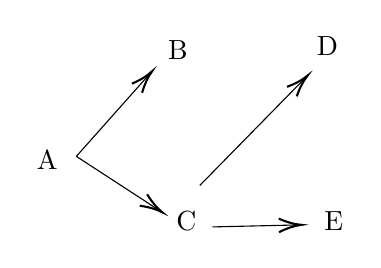
\begin{tikzpicture}[x=0.75pt,y=0.75pt,yscale=-1,xscale=1]
%uncomment if require: \path (0,193); %set diagram left start at 0, and has height of 193

%Straight Lines [id:da7671178109085042] 
\draw    (100,108) -- (135.17,68.49) ;
\draw [shift={(136.5,67)}, rotate = 491.68] [color={rgb, 255:red, 0; green, 0; blue, 0 }  ][line width=0.75]    (10.93,-3.29) .. controls (6.95,-1.4) and (3.31,-0.3) .. (0,0) .. controls (3.31,0.3) and (6.95,1.4) .. (10.93,3.29)   ;

%Straight Lines [id:da5752878963713413] 
\draw    (100,108) -- (139.82,133.91) ;
\draw [shift={(141.5,135)}, rotate = 213.05] [color={rgb, 255:red, 0; green, 0; blue, 0 }  ][line width=0.75]    (10.93,-3.29) .. controls (6.95,-1.4) and (3.31,-0.3) .. (0,0) .. controls (3.31,0.3) and (6.95,1.4) .. (10.93,3.29)   ;

%Straight Lines [id:da7032983241128152] 
\draw    (159.5,122) -- (210.1,70.43) ;
\draw [shift={(211.5,69)}, rotate = 494.45] [color={rgb, 255:red, 0; green, 0; blue, 0 }  ][line width=0.75]    (10.93,-3.29) .. controls (6.95,-1.4) and (3.31,-0.3) .. (0,0) .. controls (3.31,0.3) and (6.95,1.4) .. (10.93,3.29)   ;

%Straight Lines [id:da6110899094626818] 
\draw    (165.5,142) -- (206.5,141.05) ;
\draw [shift={(208.5,141)}, rotate = 538.6700000000001] [color={rgb, 255:red, 0; green, 0; blue, 0 }  ][line width=0.75]    (10.93,-3.29) .. controls (6.95,-1.4) and (3.31,-0.3) .. (0,0) .. controls (3.31,0.3) and (6.95,1.4) .. (10.93,3.29)   ;


% Text Node
\draw (86,110) node  [align=left] {A};
% Text Node
\draw (149,57) node  [align=left] {B};
% Text Node
\draw (153,139) node  [align=left] {C};
% Text Node
\draw (221,55) node  [align=left] {D};
% Text Node
\draw (224,139) node  [align=left] {E};


\end{tikzpicture}\\
For the graph to contain the shortest path, it would need to contain \{AB,AC,CE,BD\} or \{AB,AC,BE,CD\} , which in this case BFS cannot produce.




\end{solution}

\newpage

For the next two problems, use the following graph $G=(V,E)$. 
\begin{center}
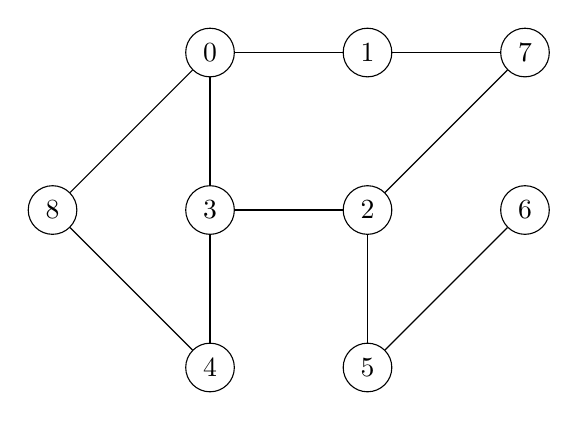
\begin{tikzpicture}[scale=2]
    \node[shape=circle,draw=black] (A0) at (2,3) {0};
    \node[shape=circle,draw=black] (A1) at (3,3) {1};
    \node[shape=circle,draw=black] (A7) at (4,3) {7};

    \node[shape=circle,draw=black] (A8) at (1,2) {8};
    \node[shape=circle,draw=black] (A3) at (2,2) {3};
    \node[shape=circle,draw=black] (A2) at (3,2) {2};
    \node[shape=circle,draw=black] (A6) at (4,2) {6};
    
    \node[shape=circle,draw=black] (A4) at (2,1) {4};
    \node[shape=circle,draw=black] (A5) at (3,1) {5};

    \draw (A8) -- (A0); 
    \draw (A8) -- (A4);  
    \draw (A0) -- (A1); 
    \draw (A0) -- (A3);
    \draw (A4) -- (A3); 
    \draw (A3) -- (A2); 
    \draw (A1) -- (A7);
    \draw (A2) -- (A7);
    \draw (A2) -- (A5);
    \draw (A5) -- (A6);  
\end{tikzpicture}
\end{center}
\begin{problem}[20 points]
Describe the order in which nodes of the graph $G$ are processed in
BFS when the start node is 8 and neighboring nodes are taking in
increasing order (smaller labels are enqueued first). 
\end{problem}
\begin{solution} \\
Processing Order
\begin{enumerate}
    \item Visit: 8   Queue: 0,4
    \item Visit: 0   Queue: 4,1,3
    \item Visit: 4   Queue: 1,3
    \item Visit: 1   Queue: 3,7
    \item Visit: 3   Queue: 7,2
    \item Visit: 7   Queue: 2
    \item Visit: 2   Queue: 5
    \item Visit: 5   Queue: 6
    \item Visit: 6   Queue: x
\end{enumerate}
Beginning at the starting node; the node is marked as visited, the adjacent nodes are queued in ascending order, and then the search moves to the next queued node.\\
\\
This makes the order of the nodes = 8,0,4,1,3,7,2,5,6\\
\end{solution}

\newpage

\begin{problem}[20 points]
Describe the order in which nodes of the graph $G$ are processed in
DFS when the start node is 8 and neighboring nodes are taking in
increasing order. 
\end{problem}
\begin{solution} \\
Depth First Search\\
\begin{enumerate}
    \item Visit: 8 Stack:
    \item Visit: 0 Stack: 8 
    \item Visit: 1 Stack: 8 0
    \item Visit: 7 Stack: 8 0 1
    \item Visit: 2 Stack: 8 0 1 7
    \item Visit: 3 Stack: 8 0 1 7 2
    \item Visit: 4 Stack: 8 0 1 7 3
    \item Visit: 3 Stack: 8 0 1 7 3 4
    \item Visit: 2 Stack: 8 0 1 7 3 4
    \item Visit: 5 Stack: 8 0 1 7 3 4
    \item Visit: 6 Stack: 8 0 1 7 3 4 5
    \item Visit: x Stack: 8 0 1 7 3 4 5 6
\end{enumerate}
Depth-first search begins at the starting node. The processed node is marked as visited. It then processes the first adjacent node (following ascending order in this case). In the case that there are no unvisited adjacent nodes, the search must backtrack through the stack, checking the conditions of each node until an unvisited adjacency appears.
\\
\\
The order of the nodes processed = 8,0,1,7,2,3,4,5,6\\
\end{solution}


% Discussions on ecampus are always encouraged, especially to clarify
% concepts that were introduced in the lecture. However, discussions of
% homework problems on ecampus should not contain spoilers. It is okay to
% ask for clarifications concerning homework questions if needed. Make
% sure that you write the solutions in your own words. 


\medskip



\goodbreak
\checklist
\end{document}
